\documentclass[11pt,a4paper,DIV=10,]{scrartcl}
\usepackage[utf8]{inputenc}
\usepackage[ngerman]{babel}
\usepackage{amsmath}
\usepackage{amsfonts}
\usepackage{amssymb}
\usepackage{fancybox}
\usepackage{multicol}
\usepackage{graphicx}
\usepackage{color}
\usepackage{colortbl}
% Define user colors using the RGB model
\definecolor{dunkelgrau}{rgb}{0.8,0.8,0.8}
\definecolor{hellgrau}{rgb}{0.95,0.95,0.95}
\usepackage[normal,font={small,color=black}, labelfont=bf,figurename=Abb.]{caption}
\usepackage{float}
\usepackage{cite}
\usepackage{url}
\bibliographystyle{unsrtnat}
\usepackage[numbers]{natbib}
%\usepackage[T1]{fontenc}


\begin{document}
\onecolumn
\subsection*{ALP4 SoSe 2013, Di. 16-18}
\section*{Lösung Übungsblatt 1}
\textbf{Christoph van Heteren-Frese (Matr.-Nr.: 4465677), \\ Sven Wildermann (Matr.-Nr.: 4567553)}\\
Tutor: Alexander Steen, eingereicht am \today\\
\hrule

\section*{Übung 1}
\subsection*{a)}
Diese Aussage ist richtig. Wenn die Reihenfolge der einzelnen Anweisungen eindeutig festgelegt sind (deterministisch), so muss bei gleichen
Eingabewerten trivialerweise auch der gleiche Ausgabewert (determiniert) geliefert  werden. 
\subsection*{b)}
Diese Aussage ist falsch. Nur weil das Ergebnis eines Algorithmusses bei gleichen Eingabewerten das selbe ist, muss die Reihenfolge der Anweisungen
nicht zwangsläufig die selbe sein. Beispiel: Das Ergebnis von zwei Additionen auf eine Variable X ist unabhängig davon welcher der beiden Additionen
zuerst ausgeführt wird. 
\subsection*{c)}
Diese Aussage stimmt, da die Sequenz eines deterministischen Algorithmus die Folge der Schritte seines Ablaufes ist. Andersherum ist da jedoch nicht der Fall. 
\subsection*{d)}
Diese Aussage ist falsch, da ein nichtsequentieller Algorithmus auch determiniert sein kann. 
Genau wie in b) kann das Ergebnis eines Algorithmusses bei gleichen Eingabewerten das selbe sein, auch wenn die Reihenfolge der Anweisungen
nicht zwangsläufig die selbe sein. Beispiel: Das Ergebnis von zwei Additionen auf eine Variable X ist unabhängig davon, ob diese zwei Operationen
zwischenzeitlich unterbrochen werden oder von mehreren Prozessoren nebenläufig ausgeführt werden (sofern die Addition atomar ist). 
\subsection*{e)}
Ein Beispiel für ein sequentiellen aber nicht determinierten Algorithmus ist ein Münzwurf. Hier erhält man bei gleichen Eingabewerten unterschiedliche Ergebnisse. Unter der Annahme dass das Ergebnis eines Zufallsexperiments nicht als Eingabe gesehen wird. 


\section*{Übung 2}
\subsection{a)}


\section*{Übung 4}
Die Ausgabe ist die Folge eines nicht sequentiellen Ablaufs der elektronischen Tafel beim Erfassen der Zeichen. So sind die gelb marktieren Threads mit den jeweiligen Zeichen für die jeweilige Spalte immer als letztes an der Reihe gewesen und haben so die vorherigen Zeichen überschrieben. Wenn man die einzlenen Sätze durchnummeriert, kann man schnell ausfindig machen welcher Prozess an welcher Stelle in der Zeichenkette zuletzt ``dran'' gewesen ist. Und zwar wie folgt: 44332255555555412244. Dabei wird deutlich, dass der Prozess Nr. 6 garnicht zum Zug gekommen ist. 

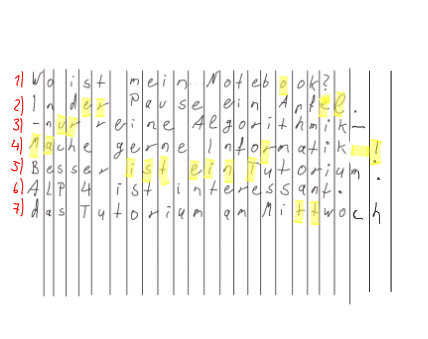
\includegraphics{picture_a4.png}

Ergebnis dieser Abfolge ist der Satz: ``Maurer ist ein Trottel !''






\end{document}